\section{Findings}
\subsection{Simulated analysis example}
\simlabel{} The current example has six blocks, 48 trials and 240,000 scheduled
slots. Its policy factors are assumptions built into the model. Table~\ref{tab:sim}
shows the 110 Mb/s, one-flow condition. The results demonstrate the reporting
path; they do not validate Linux queue behavior.

\begin{table}[htbp]\centering
\caption{Simulated example. Six paired blocks per policy.}\label{tab:sim}
\begin{tabular}{lrr}\toprule
Policy & Added on-time p99 (ms) & FIFO goodput retained (\%)\\\midrule
FIFO & 15.942 & 100.00\\
FQ-CoDel & 4.769 & 98.75\\
CAKE best-effort & 3.228 & 94.31\\
CAKE bounded & 2.550 & 95.77\\\bottomrule
\end{tabular}
\end{table}

The model includes 967 unsent slots and 108 timeout or late outcomes. Its
K-means and Ward fits have silhouette 0.212; DBSCAN finds one dense group and
labels 19 of the 24 loaded runs as noise. This disagreement is a useful warning
against treating a two-dimensional cluster picture as proof of distinct network
regimes. We keep every run. Ridge and Lasso have held-out-block MAE of 0.0358
and 0.0426 ms, respectively, compared with 4.659 ms for the training-mean
baseline. The small errors reflect a simple, deliberately structured toy
generator. They are not evidence of prediction accuracy on real traffic.

\begin{figure}[htbp]\centering
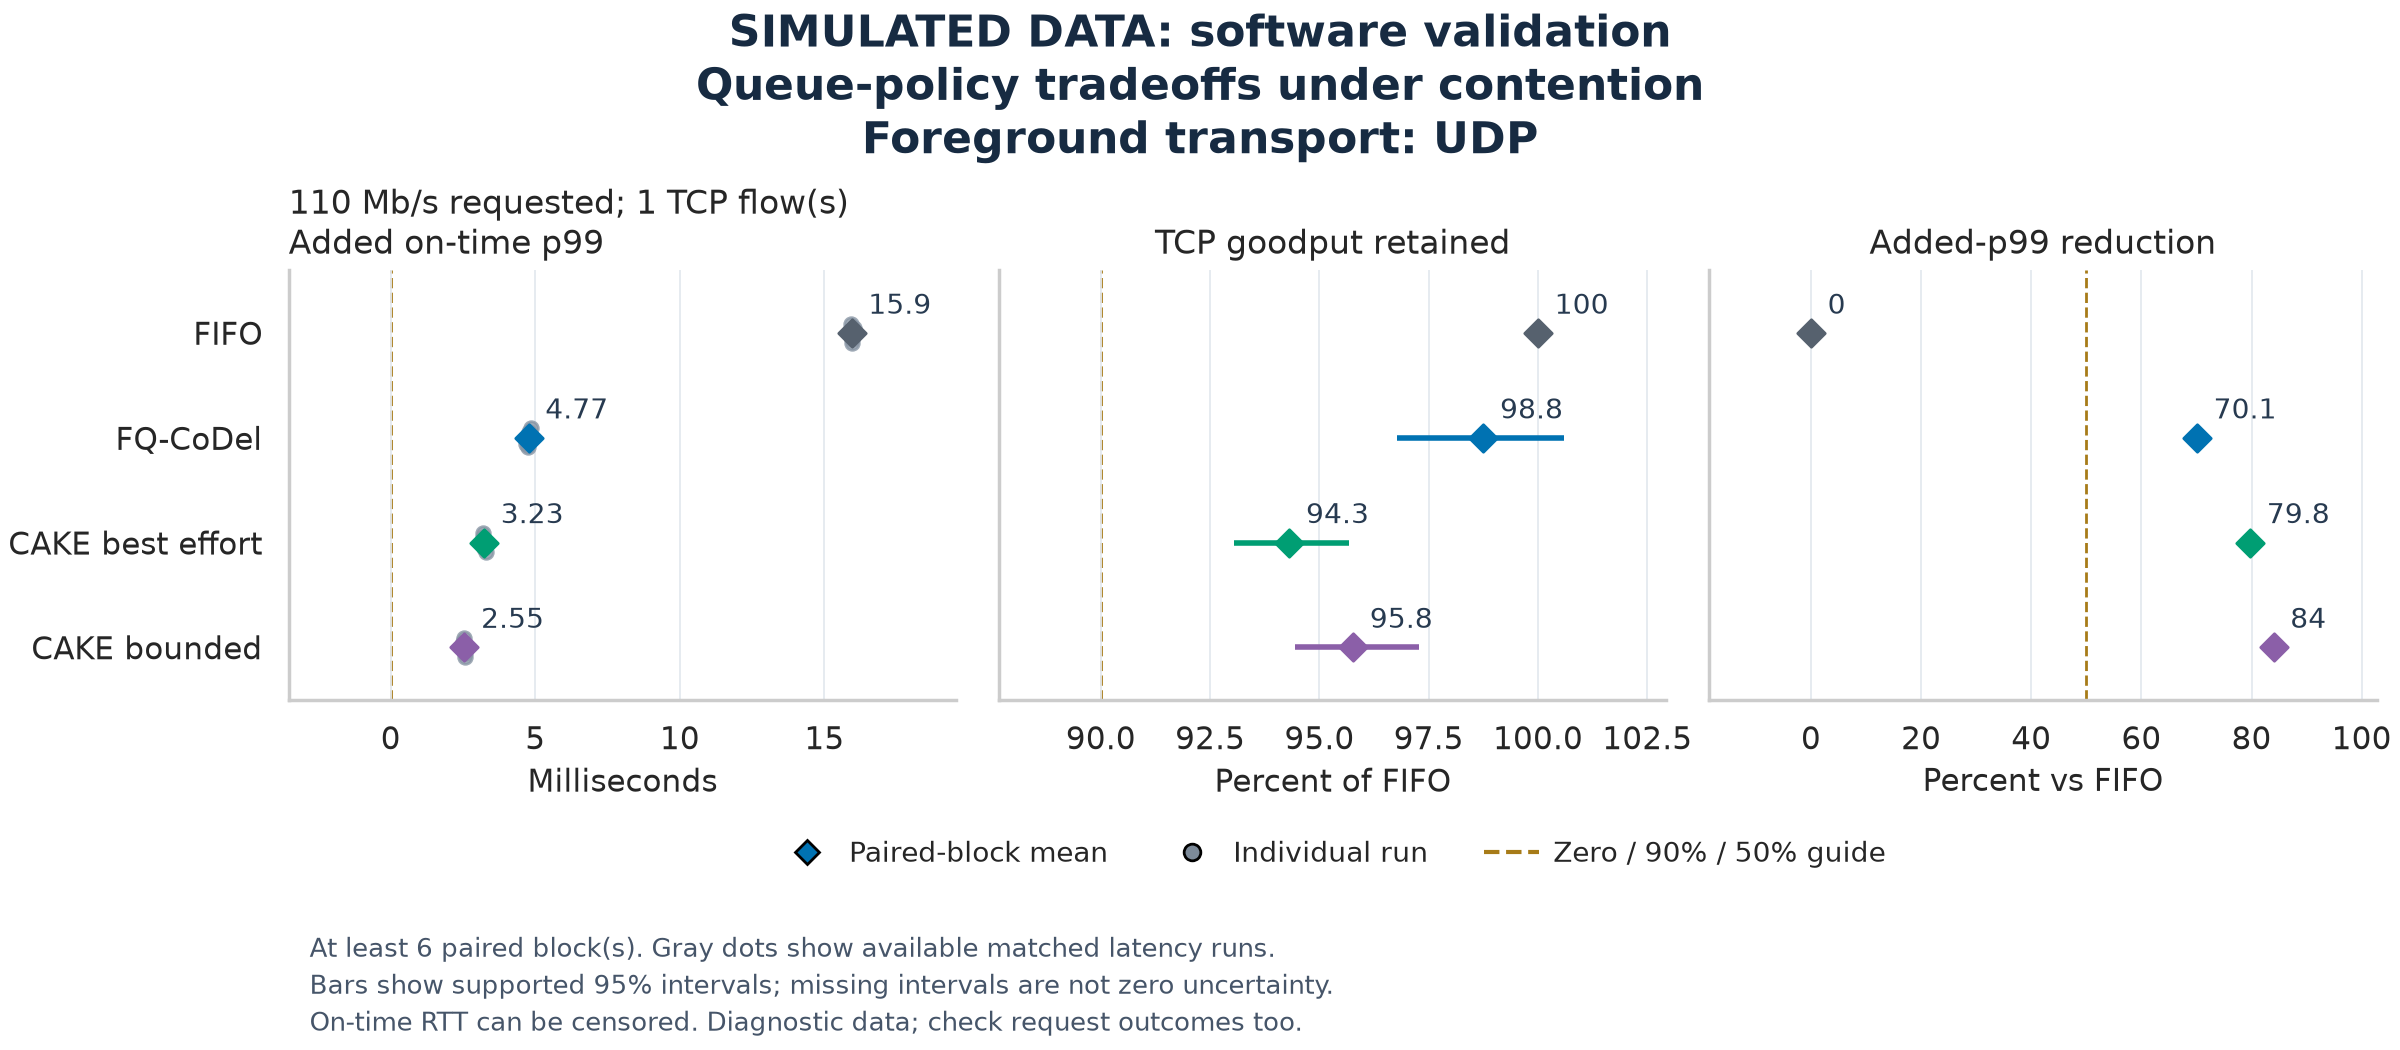
\includegraphics[width=\linewidth]{../analysis/plots/simulation/policy_comparisons.png}
\caption{Simulated policy comparison from the recorded six-block example.
Intervals describe variation in the toy model, not uncertainty about hardware.}
\end{figure}

\subsection{Existing namespace measurements}
The separate November 11 namespace pilot contains 16 completed trials and
80,000 scheduled measurement slots. It retained 3,192 unsent slots (3.99\%),
with no recorded timeout or late outcomes. Table~\ref{tab:pilot} reports the
two-block means. The analysis withholds confidence intervals because there
are too few blocks. The source is the retained e3ddaff export from hosted
Linux workflow 43111991762, available in the repository's reference directory.

\begin{table}[htbp]\centering
\caption{Observed namespace pilot, two paired blocks. No physical NucBox measurements.}\label{tab:pilot}
\begin{tabular}{lrr}\toprule
Policy & Added on-time p99 (ms) & FIFO goodput retained (\%)\\\midrule
FIFO & 18.977 & 100.00\\
FQ-CoDel & 0.104 & 99.37\\
CAKE best-effort & 0.106 & 89.37\\
CAKE bounded & 0.094 & 89.18\\\bottomrule
\end{tabular}
\end{table}

Both CAKE variants miss the 90\% goodput target in this pilot despite the
lower observed on-time p99. FQ-CoDel meets both point-estimate targets here,
but the small sample, omitted sends and shared-host environment prevent a
strong recommendation. We cannot infer that a missing request would have
experienced the same latency as a request that was sent.

\subsection{What the physical run must establish}
The NucBox/MacBook run must first establish the actual link path, base RTT,
queue attachment, offered and achieved load, and generator behavior. We will
replace the simulated comparison with the measured per-condition results,
paired intervals and outcome counts while retaining the reference example
separately. A treatment will count as feasible only if both stated targets
are supported by valid evidence, with uncertainty reported.

Exact foreground and bulk measurement-window alignment remains unresolved.
The retained iperf3 receiver interval is checked against its byte totals but
does not prove alignment with the foreground window. Router CPU is also
unavailable in the mixed endpoint collector. Native Mac TCP behavior, USB
adapter effects and the changed delay placement limit comparison with the
Linux-only pilot. We will report these limitations and any failed runs rather
than turn successful pipeline execution into a scientific success claim.
